%----------------------------------------------------------------------------------------
%	BOOK INFORMATION
%----------------------------------------------------------------------------------------

% \titlehead{Document Template}
\title[Working Title: Why did JT release the 20/20 experience in 2013?]{Working Title: Why did JT release the 20/20 experience in 2013?}
\subtitle{Doctoral Thesis}
\author[D. C. Makwana]{Dhruv C. Makwana}%
\date{\today \\[\baselineskip] 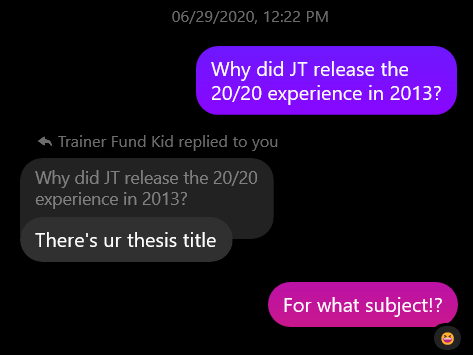
\includegraphics[width=.8\textwidth]{figures/working-title.png}
}
% \publishers{An Awesome Publisher}

%----------------------------------------------------------------------------------------

\frontmatter % Denotes the start of the pre-document content, uses roman numerals

%----------------------------------------------------------------------------------------
%	COPYRIGHT PAGE
%----------------------------------------------------------------------------------------

\makeatletter
\uppertitleback{\@titlehead} % Header

\lowertitleback{
	% \textbf{Disclaimer} \\
	% You can edit this page to suit your needs. For instance, here we have a no copyright statement, a colophon and some other information. This page is based on the corresponding page of Ken Arroyo Ohori's thesis, with minimal changes.
	
	% \medskip
	
	% \textbf{No copyright} \\
	% \cczero\ This book is released into the public domain using the CC0 code. To the extent possible under law, I waive all copyright and related or neighbouring rights to this work.
	
	% To view a copy of the CC0 code, visit: \\\url{http://creativecommons.org/publicdomain/zero/1.0/}
	
	% \medskip
	
	% \textbf{Colophon} \\
	% This document was typeset with the help of \href{https://sourceforge.net/projects/koma-script/}{\KOMAScript} and \href{https://www.latex-project.org/}{\LaTeX} using the \href{https://github.com/fmarotta/kaobook/}{kaobook} class.
	
	% \medskip
	
	% \textbf{Publisher} \\
	% First printed in May 2019 by \@publishers
}
\makeatother

%----------------------------------------------------------------------------------------
%	DEDICATION
%----------------------------------------------------------------------------------------

\dedication{\raggedleft\emph{To \_,\\
Something short and sweeet.}}

% \dedication{
% 	% The harmony of the world is made manifest in Form and Number, and the heart and soul and all the poetry of Natural Philosophy are embodied in the concept of mathematical beauty.\\
% 	% \flushright -- D'Arcy Wentworth Thompson
% }

%----------------------------------------------------------------------------------------
%	OUTPUT TITLE PAGE AND PREVIOUS
%----------------------------------------------------------------------------------------

% \includepdf[pages=1]{../MathSTICTemplate/main.pdf}

% Note that \maketitle outputs the pages before here
\maketitle

%----------------------------------------------------------------------------------------
%	PREFACE
%----------------------------------------------------------------------------------------

\begingroup

  %in the header, chapters start on any page to avoid too many blank pages
  \let\cleardoublepage\clearpage
  \pagelayout{margin}

\addchap{Abstract}

\addchap{Acknowledgments}

\addchap{How to Read This Thesis}

Use some words to talk about
\begin{itemize}
    \item lots of hyperlinking
    \item but not visible for readability
    \item example of \kl{bidirectional}
    \item in \cref{chap:kernel-cn}
    \item and emphasis like the following \intro{example}
    \item and even $\obsRef$.
\end{itemize}

Don't be confused, just click!

And also talk about the large margins, and fragments of the same figure like
\cref{fig:cic-var,fig:cic-nondep-fun}.

But still printable - colours are only (mostly?) used to aid readability.

\endgroup

%----------------------------------------------------------------------------------------
%	TABLE OF CONTENTS & LIST OF FIGURES/TABLES
%----------------------------------------------------------------------------------------

\pagelayout{wide}
\cleardoubleevenemptypage

\knowledgeconfigure{protect links}

\begingroup % Local scope for the following commands

\hypersetup{allcolors=.}

% Define the style for the TOC, LOF, and LOT
%\setstretch{1} % Uncomment to modify line spacing in the ToC
%\hypersetup{linkcolor=blue} % Uncomment to set the colour of links in the ToC
\setlength{\textheight}{230\vscale} % Manually adjust the height of the ToC pages

% Turn on compatibility mode for the etoc package
\etocstandarddisplaystyle % "toc display" as if etoc was not loaded
\etocstandardlines % "toc lines as if etoc was not loaded
\setcounter{tocdepth}{\sectiontocdepth} % Locally for the global toc

\tableofcontents % Output the table of contents

\setcounter{tocdepth}{\subsectiontocdepth} % To have correct tocs in the sections

% \listoffigures % Output the list of figures

% Comment both of the following lines to have the LOF and the LOT on different pages
% \let\cleardoublepage\bigskip
% \let\clearpage\bigskip

% \listoftables % Output the list of tables

\endgroup
\knowledgeconfigure{unprotect links}
